\documentclass[11pt,a4paper]{article}

\usepackage[utf8]{inputenc}
\usepackage[margin=2.3cm]{geometry}
\usepackage{microtype}
\usepackage{xcolor}
\usepackage{booktabs}
\usepackage{tabularx}
\usepackage{longtable}
\usepackage{array}
\usepackage{enumitem}
\usepackage{fancyhdr}
\usepackage{textcomp}
\usepackage{upquote}
\usepackage{listings}
\usepackage{tikz}
\usetikzlibrary{positioning,arrows.meta,shapes.geometric,fit,backgrounds,calc}
\usepackage[colorlinks=true,linkcolor=blue!50!black,urlcolor=blue!50!black,citecolor=blue!50!black]{hyperref}

\definecolor{brand}{HTML}{1F4E79}
\definecolor{softgray}{HTML}{F3F5F8}
\definecolor{codebg}{HTML}{F6F8FA}

\setlength{\parindent}{0pt}
\setlength{\parskip}{0.55em}
\setlist{itemsep=0.15em,topsep=0.3em}
\renewcommand{\arraystretch}{1.18}

\pagestyle{fancy}
\fancyhf{}
\fancyhead[L]{\small AnyDB CMS}
\fancyhead[R]{\small Design Documentation}
\fancyfoot[C]{\small\thepage}
\renewcommand{\headrulewidth}{0.3pt}

\newcommand{\code}[1]{\texttt{\detokenize{#1}}}

\lstdefinestyle{code}{
  basicstyle=\ttfamily\footnotesize,
  backgroundcolor=\color{codebg},
  frame=single,
  rulecolor=\color{black!15},
  breaklines=true,
  breakatwhitespace=false,
  columns=fullflexible,
  keepspaces=true,
  showstringspaces=false,
  keywordstyle=\color{brand}\bfseries,
  commentstyle=\color{black!55}\itshape,
  xleftmargin=0.3em,
  xrightmargin=0.3em,
  aboveskip=0.6em,
  belowskip=0.4em
}
\lstset{style=code}
\lstdefinelanguage{proto}{
  morekeywords={syntax,package,import,service,rpc,returns,message,repeated,stream,string,bool,int32,int64},
  morecomment=[l]{//},
  sensitive=true
}
\lstdefinelanguage{json}{
  morestring=[b]",
  string=[b]",
  literate=*{:}{{:}}1,
  sensitive=true
}

\tikzset{
  box/.style={draw=brand,rounded corners=3pt,fill=softgray,align=center,
              minimum height=0.9cm,inner sep=4pt,font=\small},
  sbox/.style={draw=black!50,rounded corners=3pt,fill=white,align=center,
               minimum height=0.8cm,inner sep=3pt,font=\footnotesize},
  db/.style={draw=black!60,cylinder,shape border rotate=90,aspect=0.25,
             fill=white,align=center,font=\footnotesize,minimum height=1.1cm,minimum width=2.1cm},
  arr/.style={-{Stealth[length=2.2mm]},draw=black!70},
  darr/.style={-{Stealth[length=2.2mm]},draw=black!70,dashed}
}

\title{\textbf{AnyDB CMS}\\[0.4em]\large One CMS for every database\\[1.2em]\normalsize Design Documentation}
\author{}
\date{Draft \textemdash{} October 2026}

\begin{document}
\maketitle
\thispagestyle{empty}

\begin{abstract}
\noindent AnyDB CMS is a database-agnostic CMS and admin layer. It connects to SQL, document, key-value and realtime databases, including cloud-hosted ones such as Firebase, Supabase, Neon, MongoDB Atlas, AWS, Google Cloud and Azure, and gives every client stack one REST/GraphQL API and one admin UI.

\medskip
\noindent\textbf{Status:} design phase. This document describes what to build and why. Nothing described here is implemented yet. ``anydbcms'' is a working name; check domain, package scope and trademark before committing. Time and file-count figures are planning estimates, not benchmarks.
\end{abstract}

\tableofcontents
\newpage

%--------------------------------------------------------------------
\section{Overview}

\subsection{Problem}
Content tools are tied to one database. Strapi and Directus are SQL-only, FireCMS is Firestore-first, and internal-tool builders such as Retool and Appsmith reach many databases but are not content CMSs. Teams running several stacks end up with several admin panels.

\subsection{Product}
AnyDB CMS is a database-agnostic CMS and admin layer:
\begin{itemize}
  \item Connect any supported database, including bring-your-own cloud databases.
  \item Introspect it, describe it as a canonical content model, and edit it through one admin UI.
  \item Expose one REST/GraphQL API so every client stack uses the same contract.
  \item Keep credentials server-side, read-only by default, with a full audit trail.
\end{itemize}

\subsection{Users}
\begin{tabularx}{\linewidth}{@{}lX@{}}
\toprule
\textbf{User} & \textbf{Needs}\\
\midrule
Developer & Connect a database, get an API and SDK\\
Editor & Edit content without touching the database\\
Admin / security & Control who sees what, rotate credentials, read audit logs\\
Tenant (multi-tenant mode) & Bring their own database safely\\
\bottomrule
\end{tabularx}\smallskip

\subsection{Scope}
\textbf{In scope for the MVP:}
\begin{itemize}
  \item Adapters: Postgres, MySQL, MongoDB, Firestore, SQL Server, DynamoDB.
  \item Introspection, content-model overlay, CRUD, cursor pagination.
  \item RBAC with field and row rules, SSO/OIDC.
  \item Encrypted credential vault, audit log, SSRF guard.
  \item REST, GraphQL and OpenAPI; a TypeScript SDK and generated Dart and Python SDKs.
  \item Admin UI.
\end{itemize}
\textbf{Later:} Cosmos DB, Spanner, BigQuery, Redshift, Redis, Firebase RTDB, realtime subscriptions across all adapters, gRPC, and adapters in other languages through the adapter protocol.

\textbf{Non-goals:}
\begin{itemize}
  \item Not a database or migration tool. It reads and writes the customer's database; it does not replace it.
  \item Not a cross-database transaction manager. Cross-source relations are resolved at the gateway, not made atomic.
  \item Not a BI or analytics tool. Warehouse adapters (BigQuery, Redshift) are read-only by default.
\end{itemize}

\subsection{Principles}
\begin{enumerate}
  \item \textbf{Security first.} Credentials never reach a browser or mobile app.
  \item \textbf{Honest capabilities.} Each adapter declares what it can and cannot do; the UI follows it.
  \item \textbf{Adapters are isolated.} One slow or hostile database cannot starve the rest.
  \item \textbf{One contract.} Clients never talk to a database directly.
\end{enumerate}

%--------------------------------------------------------------------
\section{What to Build}

\subsection{Components}
\begin{longtable}{@{}p{5.9cm}p{8.3cm}c@{}}
\toprule
\textbf{Component} & \textbf{Purpose} & \textbf{MVP}\\
\midrule
\endhead
\code{packages/core} & Canonical content model, query AST, capability flags, errors & Yes\\
\code{protocol/} & Language-neutral adapter contract (proto and OpenAPI) & Yes\\
\code{packages/adapter-sdk} & Base adapter, registry, conformance test kit & Yes\\
\code{packages/adapters/*} & One adapter per database & 6\\
\code{packages/vault} & Envelope encryption, KMS, key rotation, cloud-identity tokens & Yes\\
\code{packages/auth} & OIDC, RBAC/ABAC, field and row rules & Yes\\
\code{packages/audit} & Append-only audit writer with redaction & Yes\\
\code{packages/network-guard} & SSRF blocklist, TLS rules, egress and tunnels & Yes\\
\code{apps/api} & Gateway: REST, GraphQL, OpenAPI & Yes\\
\code{apps/worker} & Isolated adapter runners, introspection jobs, realtime & Yes\\
\code{apps/admin} & Editor and admin UI & Yes\\
\code{db/control-plane} & Migrations for tenants, connections, metadata, permissions, audit & Yes\\
\code{sdk-ts} & Hand-tuned TypeScript client & Yes\\
\code{sdks/dart}, \code{sdks/python} & Generated from OpenAPI plus a small hand-written layer & Yes\\
\code{infra/} & Docker, Terraform, Kubernetes & Yes\\
\code{tests/} & Conformance, security, end-to-end & Yes\\
\bottomrule
\end{longtable}

\subsection{Adapter families}
\begin{tabularx}{\linewidth}{@{}l>{\raggedright\arraybackslash}p{4.2cm}X@{}}
\toprule
\textbf{Family} & \textbf{Adapters} & \textbf{Notes}\\
\midrule
SQL & postgres, mysql, mssql & postgres covers Supabase, Neon, RDS, Aurora, Cloud SQL, AlloyDB, Azure PostgreSQL\\
Document & mongodb, firestore, cosmosdb & mongodb also covers Atlas, DocumentDB (feature gaps), Cosmos Mongo API\\
Key-value & dynamodb, redis & Key conditions only; scans are explicit and costly\\
Realtime & firebase-rtdb & Path-based\\
Analytics & bigquery, redshift & Read-only by default; later\\
Other cloud & spanner, athena, opensearch & Later, on demand\\
\bottomrule
\end{tabularx}\smallskip

\subsection{Per-adapter files}
Every adapter folder has the same layout, so adding a database is a copy-and-fill job:
\begin{lstlisting}
package.json  tsconfig.json  README.md
src/index.ts  adapter.ts  config.schema.ts  connection.ts  auth.ts
src/introspect.ts  capabilities.ts  query-compiler.ts  type-map.ts
src/operations.ts  pagination.ts  realtime.ts  errors.ts
tests/conformance.test.ts  compiler.test.ts  introspect.test.ts  security.test.ts
\end{lstlisting}

\subsection{Dependency rules (enforced in CI)}
\begin{itemize}
  \item \code{core} imports nothing internal.
  \item \code{adapters/*} depend only on \code{core} and \code{adapter-sdk}.
  \item \code{admin} talks only to \code{api} or \code{sdk-ts}, never to a database.
  \item Only \code{api} and \code{worker} may import \code{vault}.
\end{itemize}

\subsection{Definition of done for an adapter}
\begin{enumerate}
  \item Passes the shared conformance suite.
  \item Passes the security suite (injection, identifier allowlist).
  \item Declares accurate capability flags.
  \item Documents supported services, auth modes and limits in its README.
\end{enumerate}

%--------------------------------------------------------------------
\section{Language Decision}
This is a recommendation based on the project's needs, not a measured benchmark.

\subsection{Recommendation}
Use \textbf{TypeScript for the whole MVP}. Add \textbf{Go} later for performance-critical or third-party adapters through the adapter protocol. Dart and Python SDKs are generated from OpenAPI.

\begin{tabularx}{\linewidth}{@{}>{\raggedright\arraybackslash}p{4.3cm}>{\raggedright\arraybackslash}p{3.3cm}X@{}}
\toprule
\textbf{Part} & \textbf{Language} & \textbf{Why}\\
\midrule
core, adapter-sdk, api, worker & TypeScript (Node.js) & One language across server and UI, shared types, strong official SDKs for Firestore, MongoDB, DynamoDB, Postgres\\
Admin UI & TypeScript, React (Refine) & Backend-agnostic data providers, same types as the API\\
Control-plane migrations & SQL & Plain and reviewable\\
SDK: TypeScript & TypeScript & Hand-tuned, first class\\
SDK: Flutter & Dart & Generated plus a small hand-written layer\\
SDK: Python & Python & Generated plus a small hand-written layer\\
Third-party or heavy adapters (later) & Go or any language & Separate process through the protocol\\
\bottomrule
\end{tabularx}\smallskip

\subsection{Why TypeScript first}
\begin{itemize}
  \item The query AST, content model and capability flags are shared by the gateway, adapters, SDK and admin UI. One type system avoids drift.
  \item Database SDK coverage is best on Node for the targets that matter (Firebase Admin, MongoDB, DynamoDB, \code{pg}/\code{mysql2}, Azure and Google clients).
  \item It is the fastest path to a working MVP for one or two engineers.
\end{itemize}

\subsection{Where TypeScript is weaker}
\begin{itemize}
  \item CPU-heavy work and very high connection counts are better in Go or Rust.
  \item A single event loop needs care: run adapters in worker processes, not inside the API process.
\end{itemize}

\subsection{Options compared}
\begin{tabularx}{\linewidth}{@{}>{\raggedright\arraybackslash}p{2.8cm}>{\raggedright\arraybackslash}p{4.0cm}>{\raggedright\arraybackslash}p{3.8cm}X@{}}
\toprule
\textbf{Option} & \textbf{Strength} & \textbf{Weakness} & \textbf{Verdict}\\
\midrule
TypeScript everywhere & Shared types, fastest MVP, best DB SDK coverage & Weaker for CPU-bound work & \textbf{MVP choice}\\
Go core & Fast, small binaries, great concurrency & Admin UI still needs TypeScript; two type systems & Good for later adapters\\
Python core & Rich data libraries & Slower, weaker typing for a gateway & SDK and scripting only\\
Rust core & Performance and safety & Slow to build, thin cloud-SDK coverage & Not worth it for the MVP\\
Java / Kotlin & Mature DB drivers & Heavier, slower iteration & Only if a client requires it\\
\bottomrule
\end{tabularx}\smallskip

\subsection{Language freedom for adapters}
Adapters run as separate processes speaking the protocol in \code{adapter.proto}. The gateway does not care what language an adapter is written in. First-party adapters ship in TypeScript and run through the same protocol, with an in-process fast path allowed for trusted ones.

%--------------------------------------------------------------------
\section{Architecture}

\subsection{System context}
\begin{figure}[h]
\centering
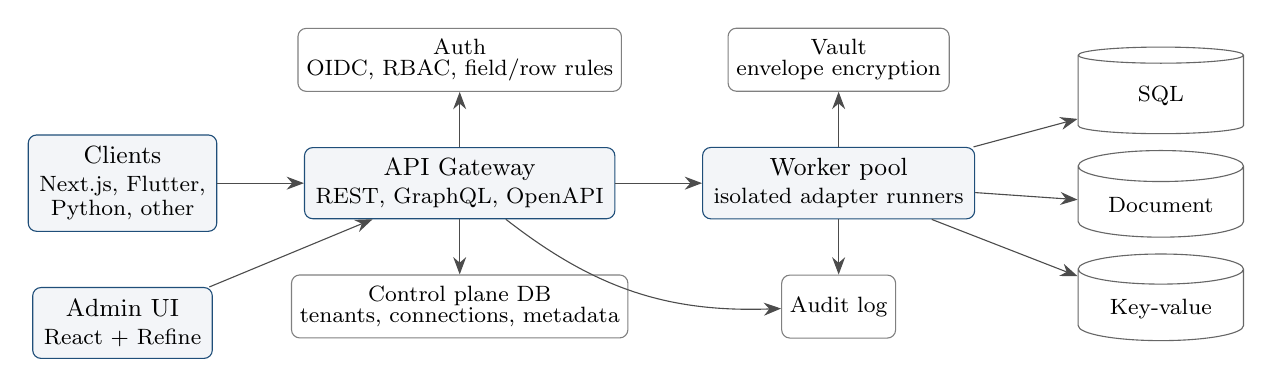
\begin{tikzpicture}[node distance=7mm and 11mm]
  \node[box] (clients) {Clients\\[-1pt]\footnotesize Next.js, Flutter,\\[-2pt]\footnotesize Python, other};
  \node[box,below=of clients] (admin) {Admin UI\\[-1pt]\footnotesize React + Refine};
  \node[box,right=of clients] (gw) {API Gateway\\[-1pt]\footnotesize REST, GraphQL, OpenAPI};
  \node[sbox,above=of gw] (auth) {Auth\\[-2pt]\footnotesize OIDC, RBAC, field/row rules};
  \node[sbox,below=of gw] (cp) {Control plane DB\\[-2pt]\footnotesize tenants, connections, metadata};
  \node[box,right=of gw] (wk) {Worker pool\\[-1pt]\footnotesize isolated adapter runners};
  \node[sbox,above=of wk] (vlt) {Vault\\[-2pt]\footnotesize envelope encryption};
  \node[sbox,below=of wk] (aud) {Audit log};
  \node[db,right=of wk,xshift=2mm,yshift=11mm] (sql) {SQL};
  \node[db,below=2mm of sql] (doc) {Document};
  \node[db,below=2mm of doc] (kv) {Key-value};

  \draw[arr] (clients) -- (gw);
  \draw[arr] (admin) -- (gw);
  \draw[arr] (gw) -- (auth);
  \draw[arr] (gw) -- (cp);
  \draw[arr] (gw) -- (wk);
  \draw[arr] (wk) -- (vlt);
  \draw[arr] (gw) to[bend right=20] (aud);
  \draw[arr] (wk) -- (aud);
  \draw[arr] (wk) -- (sql);
  \draw[arr] (wk) -- (doc);
  \draw[arr] (wk) -- (kv);
\end{tikzpicture}
\caption{System context. Clients and the admin UI only ever call the gateway.}
\end{figure}

\subsection{Layers}
\begin{figure}[h]
\centering
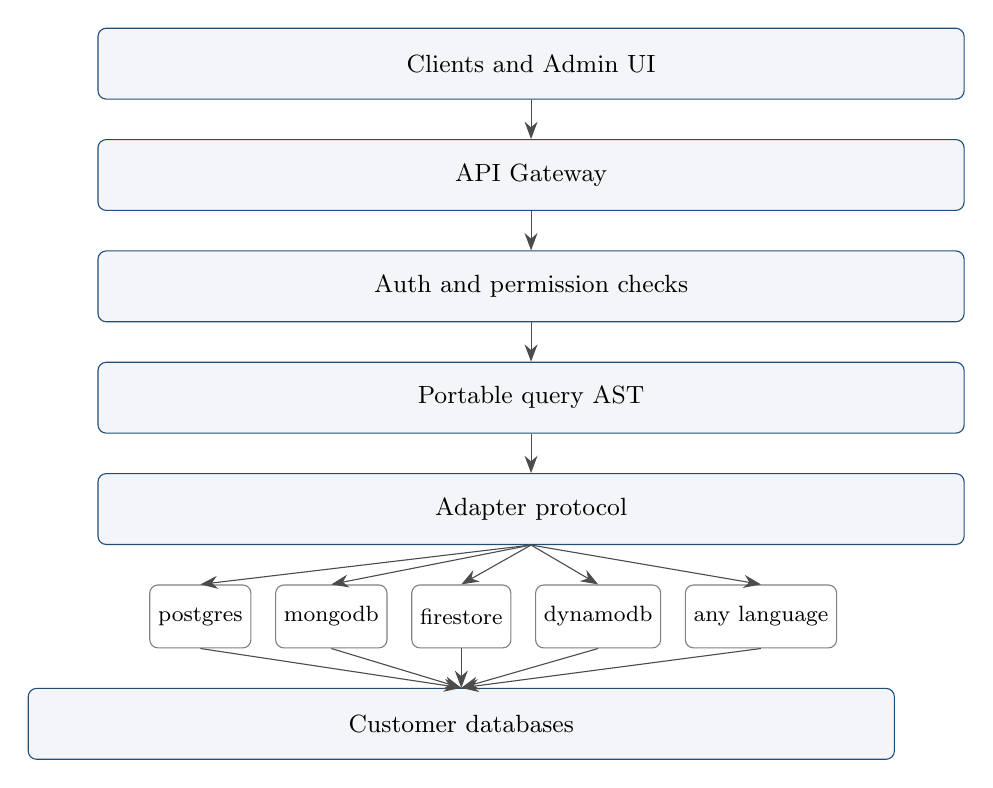
\begin{tikzpicture}[node distance=5mm]
  \node[box,minimum width=11cm] (a) {Clients and Admin UI};
  \node[box,minimum width=11cm,below=of a] (b) {API Gateway};
  \node[box,minimum width=11cm,below=of b] (c) {Auth and permission checks};
  \node[box,minimum width=11cm,below=of c] (d) {Portable query AST};
  \node[box,minimum width=11cm,below=of d] (e) {Adapter protocol};
  \node[sbox,below=of e,xshift=-4.2cm] (f1) {postgres};
  \node[sbox,right=3mm of f1] (f2) {mongodb};
  \node[sbox,right=3mm of f2] (f3) {firestore};
  \node[sbox,right=3mm of f3] (f4) {dynamodb};
  \node[sbox,right=3mm of f4] (f5) {any language};
  \node[box,minimum width=11cm,below=of f3] (g) {Customer databases};
  \foreach \s/\t in {a/b,b/c,c/d,d/e}{\draw[arr] (\s) -- (\t);}
  \foreach \f in {f1,f2,f3,f4,f5}{\draw[arr] (e.south) -- (\f.north); \draw[arr] (\f.south) -- (g.north);}
\end{tikzpicture}
\caption{Request path from client to database.}
\end{figure}

\subsection{Read request flow}
\begin{enumerate}
  \item The client calls \code{GET /v1/connections/{id}/collections/orders/records}.
  \item The gateway verifies the token and resolves roles through Auth.
  \item The gateway loads connection and collection metadata from the control plane.
  \item It builds the query AST and applies field and row rules.
  \item It calls \code{find(ast)} on the worker over the adapter protocol.
  \item The worker fetches a short-lived credential or IAM token from the vault.
  \item The adapter runs a parameterised native query against the customer database.
  \item The worker returns records and a next cursor; the gateway appends an audit event and responds.
\end{enumerate}

\subsection{Connect-and-introspect flow}
\begin{enumerate}
  \item An admin posts a new connection (type, host, secret reference).
  \item The network guard validates the host (SSRF, TLS, allowlist).
  \item The vault encrypts and stores the secret.
  \item The control plane saves the connection, read-only by default.
  \item A worker reads the catalog or samples documents and saves a draft content model.
  \item The admin reviews the draft schema before any collection is exposed.
\end{enumerate}

\subsection{Capability handling}
When a query uses something an adapter cannot do, the gateway has three outcomes: compile it to the native query (supported), reject it with \code{CAPABILITY_UNSUPPORTED} (not supported), or emulate it at the gateway and flag it in the response (emulatable). For example, DynamoDB has no arbitrary sort, so sorting by any column is rejected; Firestore has limited OR and inequality filters, so some filters are rejected or emulated and marked as such.

\subsection{Multi-tenant bring-your-own-database}
The control plane holds tenants, connections, secret references, collection metadata, and roles. The data plane runs one isolated worker per connection (or per tenant). Each connection gets its own pool limits so one tenant's slow query cannot starve another.

\subsection{Deployment view}
A load balancer with a WAF fronts stateless API pods. API pods use the control-plane Postgres and a job queue. Worker pods read secrets through KMS and reach customer databases through a NAT with static egress IPs, so customers can allowlist the platform. Private networking (PrivateLink, Private Service Connect, Azure Private Link) and SSH tunnels are supported alongside.

%--------------------------------------------------------------------
\section{Adapter Contract}
An adapter is the only code that knows a database's native language. It turns the portable query AST into native queries and native results into canonical records.

\subsection{Required operations}
\begin{tabularx}{\linewidth}{@{}>{\raggedright\arraybackslash}p{4.0cm}X@{}}
\toprule
\textbf{Operation} & \textbf{Purpose}\\
\midrule
\code{connect(config)} & Open a connection or client using resolved credentials\\
\code{introspect()} & Return collections, fields, types, keys, relations, indexes\\
\code{capabilities()} & Return capability flags\\
\code{find(query)} & List records by filter, sort, projection, cursor\\
\code{get(collection, id)} & Fetch one record\\
\code{create / update / delete} & Write operations (blocked on read-only connections)\\
\code{batch(ops)} & Multiple writes, atomic only if \code{transactions} is supported\\
\code{subscribe(query)} & Optional realtime stream\\
\code{close()} & Release resources\\
\bottomrule
\end{tabularx}\smallskip

\subsection{Capability flags}
\begin{lstlisting}[language={}]
interface Capabilities {
  joins: boolean;
  transactions: "none" | "single-document" | "multi-document";
  filters: { or: boolean; inequality: "full" | "single-field" | "none";
             fullText: boolean };
  sort: "any-field" | "indexed-only" | "key-only";
  pagination: { cursor: true; offset: boolean };   // cursor is mandatory
  aggregations: boolean;
  realtime: boolean;
  schema: "enforced" | "inferred";
  writes: boolean;
}
\end{lstlisting}
The gateway and admin UI use these flags to hide or disable unsupported controls instead of doing silent client-side work.

\subsection{Mapping rules per family}
\begin{tabularx}{\linewidth}{@{}>{\raggedright\arraybackslash}p{2.4cm}>{\raggedright\arraybackslash}p{3.8cm}>{\raggedright\arraybackslash}p{4.0cm}X@{}}
\toprule
\textbf{Concern} & \textbf{SQL} & \textbf{Document} & \textbf{Key-value}\\
\midrule
Introspection & Read catalog (information\_schema) & Sample documents, infer draft schema & Read key schema, sample items\\
Filters & Parameterised SQL & Native filter objects & Key conditions only\\
Pagination & Keyset & startAfter cursor & LastEvaluatedKey\\
Relations & Foreign keys & Reference fields or embedding & Denormalised\\
Transactions & Full & Limited & Limited\\
\bottomrule
\end{tabularx}\smallskip

\subsection{Error model}
Adapters map native errors to a fixed set so clients see one vocabulary: \code{CONNECTION_FAILED}, \code{AUTH_FAILED}, \code{NOT_FOUND}, \code{CONFLICT}, \code{VALIDATION_FAILED}, \code{CAPABILITY_UNSUPPORTED}, \code{RATE_LIMITED}, \code{TIMEOUT}, \code{READ_ONLY}, \code{INTERNAL}.

\subsection{Conformance suite}
A shared test kit runs the same scenarios against every adapter:
\begin{enumerate}
  \item introspect returns stable collections and field types;
  \item create, get, update, delete round trip;
  \item cursor pagination returns each record exactly once;
  \item unsupported filters return \code{CAPABILITY_UNSUPPORTED};
  \item a read-only connection rejects writes with \code{READ_ONLY};
  \item hostile identifiers and operators are rejected (injection);
  \item errors map to the standard set.
\end{enumerate}
An adapter is not releasable until all pass.

\subsection{Adding a new adapter}
Copy the adapter template; fill in the config schema, connection, introspection, query compiler and type map; declare capabilities honestly; register it in the registry; pass the conformance and security suites. Nothing in core, api or admin changes.

%--------------------------------------------------------------------
\section{Data Model and Schemas}
Two models exist and must not be mixed. The \textbf{control plane} is the platform's own Postgres database (tenants, connections, metadata, permissions, audit). The \textbf{canonical content model} is the platform's description of a customer's data; it is stored in the control plane, never inside the customer's database.

\subsection{Control-plane entities}
\begin{figure}[t]
\centering
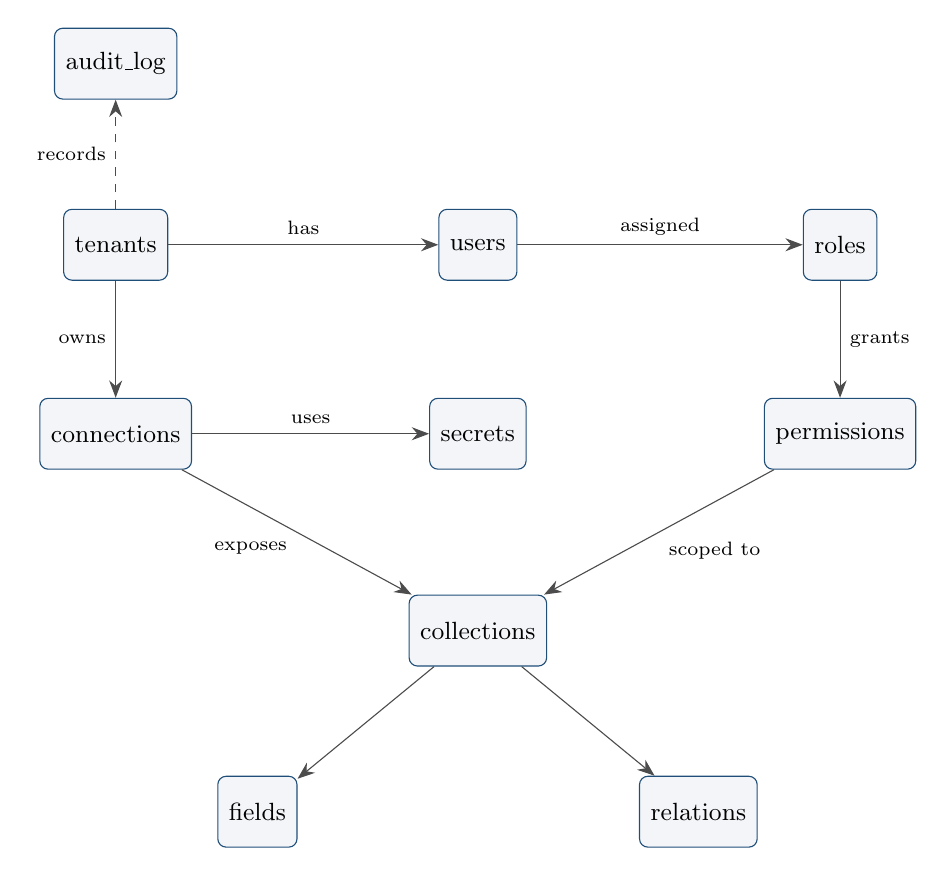
\begin{tikzpicture}
  \node[box] (tenants) at (0,0) {tenants};
  \node[box] (users) at (4.6,0) {users};
  \node[box] (roles) at (9.2,0) {roles};
  \node[box] (conn) at (0,-2.4) {connections};
  \node[box] (sec) at (4.6,-2.4) {secrets};
  \node[box] (perm) at (9.2,-2.4) {permissions};
  \node[box] (coll) at (4.6,-4.9) {collections};
  \node[box] (fields) at (1.8,-7.2) {fields};
  \node[box] (rel) at (7.4,-7.2) {relations};
  \node[box] (audit) at (0,2.3) {audit\_log};

  \draw[arr] (tenants) -- node[above,font=\scriptsize]{has} (users);
  \draw[arr] (users) -- node[above,font=\scriptsize]{assigned} (roles);
  \draw[arr] (roles) -- node[right,font=\scriptsize]{grants} (perm);
  \draw[arr] (tenants) -- node[left,font=\scriptsize]{owns} (conn);
  \draw[arr] (conn) -- node[above,font=\scriptsize]{uses} (sec);
  \draw[arr] (conn) -- node[below left,font=\scriptsize]{exposes} (coll);
  \draw[arr] (perm) -- node[below right,font=\scriptsize]{scoped to} (coll);
  \draw[arr] (coll) -- (fields);
  \draw[arr] (coll) -- (rel);
  \draw[darr] (tenants) -- node[left,font=\scriptsize]{records} (audit);
\end{tikzpicture}
\caption{Control-plane entities. The full DDL follows in Section~\ref{sec:ddl}.}
\end{figure}

\subsection{Canonical content model}
A \textbf{collection} has a name, a native name, fields, relations and capabilities. A \textbf{field} has a name, a canonical type, \emph{required} and \emph{unique} flags, validation rules and UI hints. A \textbf{relation} has a name, a kind and a mapping to a target collection. Canonical types: string, text, integer, decimal, boolean, datetime, date, json, array, reference, binary, geopoint.

\subsection{Type mapping (canonical to native)}
\begin{tabularx}{\linewidth}{@{}>{\raggedright\arraybackslash}p{1.8cm}>{\raggedright\arraybackslash}p{2.6cm}>{\raggedright\arraybackslash}p{2.1cm}>{\raggedright\arraybackslash}p{2.3cm}>{\raggedright\arraybackslash}p{2.3cm}X@{}}
\toprule
\textbf{Canonical} & \textbf{Postgres} & \textbf{MySQL} & \textbf{MongoDB} & \textbf{Firestore} & \textbf{DynamoDB}\\
\midrule
string & varchar/text & varchar & string & string & S\\
integer & int/bigint & int/bigint & int32/int64 & integer & N\\
decimal & numeric & decimal & decimal128 & double & N\\
boolean & boolean & tinyint(1) & bool & boolean & BOOL\\
datetime & timestamptz & datetime & date & timestamp & S (ISO) or N\\
json & jsonb & json & object & map & M\\
array & array or jsonb & json & array & array & L\\
reference & foreign key & foreign key & ObjectId & document ref & key string\\
geopoint & point & point & GeoJSON & geopoint & M\\
\bottomrule
\end{tabularx}\smallskip

Adapters own the exact conversion in \code{type-map.ts}. Lossy conversions must be flagged during introspection.

\subsection{Portable query AST}
A query has a collection, an optional filter (\code{and}/\code{or}/\code{not} over comparisons), sort, projection and a page (limit and cursor). Comparison operators: \code{eq, ne, lt, lte, gt, gte, in, nin, contains, startsWith, exists}.
\begin{lstlisting}[language=json]
{
  "collection": "orders",
  "filter": { "and": [
    { "field": "status", "op": "eq", "value": "paid" },
    { "field": "total", "op": "gte", "value": 100 }
  ]},
  "sort": [{ "field": "created_at", "dir": "desc" }],
  "projection": ["id", "status", "total", "created_at"],
  "page": { "limit": 50, "cursor": null }
}
\end{lstlisting}
Field names are always validated against introspected metadata before compilation; they are never interpolated into native queries.

\subsection{Rules}
\begin{enumerate}
  \item Metadata lives in the control plane, never in the customer's database.
  \item Cursor pagination is the default everywhere.
  \item Cross-source relations resolve at the gateway with batching, not inside any database.
  \item Validation happens in the CMS layer for schemaless stores.
\end{enumerate}

\subsection{Control-plane DDL}\label{sec:ddl}
\lstinputlisting[language=SQL]{../schemas/control-plane.sql}

\subsection{Query AST JSON Schema}
\lstinputlisting[language=json]{../schemas/query-ast.schema.json}

%--------------------------------------------------------------------
\section{Security}
Security drives the architecture. This section lists the controls the MVP must have.

\subsection{Threat model}
\begin{tabularx}{\linewidth}{@{}>{\raggedright\arraybackslash}p{5.0cm}X@{}}
\toprule
\textbf{Threat} & \textbf{Control}\\
\midrule
Stolen credentials from the control plane & Envelope encryption; key held in KMS, not in the database\\
Credentials leaking to clients & Clients only call the API; secrets never leave the vault\\
SSRF through bring-your-own-database hosts & Block private ranges and metadata endpoints unless explicitly configured\\
Query injection & Parameterised queries, identifier allowlist from introspected metadata, operator allowlist\\
Over-broad database access & Dedicated least-privilege role, read-only by default\\
Cross-tenant impact & Isolated workers, per-connection pool and rate limits\\
Unaccountable changes & Append-only audit log outside tenant databases\\
\bottomrule
\end{tabularx}\smallskip

\subsection{Credentials}
\begin{itemize}
  \item Encrypt connection secrets with a data key wrapped by a KMS key (envelope encryption), with a documented rotation path.
  \item Back up the key separately from database backups. Losing it makes secrets unrecoverable.
  \item Prefer identity-based access over stored passwords: AWS IAM database auth, cross-account roles with external ID and Secrets Manager ARNs; Google service accounts, the Cloud SQL connector and IAM database auth; Azure Entra ID tokens and managed identities (tokens expire, so the vault refreshes them).
  \item Never log secrets. Redact connection strings in errors.
\end{itemize}

\subsection{Least privilege}
\begin{itemize}
  \item Ask tenants for a dedicated CMS role scoped to the needed schemas or tables.
  \item Connections are \textbf{read-only by default}; write mode is an explicit opt-in.
  \item \textbf{Firebase:} the Admin SDK uses a service account with full access and is not gated by Security Rules. Scope the service account with IAM and enforce authorization in the CMS.
  \item \textbf{Supabase:} the service-role key bypasses row-level security. To enforce RLS, forward the editor's JWT or use a dedicated Postgres role.
\end{itemize}

\subsection{Network controls}
\begin{itemize}
  \item Require TLS (\code{verify-full} where supported); allow custom CA bundles.
  \item Publish static egress IPs so tenants can allowlist the platform.
  \item Support SSH tunnels and private networking.
  \item Resolve and validate hostnames server-side and re-check after DNS resolution to avoid rebinding.
\end{itemize}

\subsection{Injection defence}
\begin{itemize}
  \item Compile the query AST to parameterised queries only.
  \item Allowlist table and column names against introspected metadata.
  \item MongoDB: reject operator injection (\code{$where}, \code{$function}, keys starting with \code{$} from user input).
  \item Firestore and DynamoDB: validate field paths.
  \item Raw-query features sit behind a separate permission and are always audited.
\end{itemize}

\subsection{Access control, audit and testing}
SSO/OIDC for editors and MFA for admins. RBAC at collection level plus field rules (hide, mask, read-only) and row filters, enforced in the gateway independently of database grants. The audit log is append-only and stored in the control plane; it records actor, tenant, connection, collection, record id, operation, a redacted diff, IP and timestamp, and also logs connection changes, credential reads by workers and permission changes.

The security test suite covers SQL and NoSQL injection, identifier allowlist bypass, SSRF (private IPs, metadata IPs, DNS rebinding), permission bypass, secret leakage in logs and errors, and cross-tenant access. CI generates an SBOM, pins dependencies and scans them on every pull request.

%--------------------------------------------------------------------
\section{API}
One contract for every client. REST is the primary surface; GraphQL is generated from the same content model; OpenAPI is the source for SDK generation.

\subsection{REST endpoints (v1)}
\begin{longtable}{@{}l>{\raggedright\arraybackslash}p{9.3cm}>{\raggedright\arraybackslash}p{4.0cm}@{}}
\toprule
\textbf{Method} & \textbf{Path} & \textbf{Purpose}\\
\midrule
\endhead
POST & \code{/v1/connections} & Create a connection (read-only by default)\\
GET & \code{/v1/connections} & List connections\\
GET & \code{/v1/connections/{id}} & Connection detail and health\\
PATCH & \code{/v1/connections/{id}} & Update config, mode, secret reference\\
DELETE & \code{/v1/connections/{id}} & Remove connection and secret\\
POST & \code{/v1/connections/{id}/introspect} & Start an introspection job\\
GET & \code{/v1/connections/{id}/collections} & List collections and fields\\
PATCH & \code{/v1/collections/{id}} & Edit display name, UI hints, exposure\\
GET & \code{/v1/connections/{id}/collections/{name}/records} & List records\\
GET & \code{.../records/{rid}} & Get one record\\
POST & \code{.../records} & Create\\
PATCH & \code{.../records/{rid}} & Update\\
DELETE & \code{.../records/{rid}} & Delete\\
POST & \code{/v1/connections/{id}/batch} & Batch writes\\
GET & \code{/v1/audit} & Query the audit log\\
GET & \code{/v1/health} & Liveness and readiness\\
\bottomrule
\end{longtable}
Write endpoints return \code{READ_ONLY} on read-only connections.

\subsection{Pagination, errors and versioning}
Pagination is cursor-only. Cursors are opaque, signed and bound to the query, so a client cannot alter the filter between pages. Offset pagination is offered only where the adapter supports it. Responses carry \code{capabilityNotes} listing any emulated or degraded behaviour.

\begin{tabularx}{\linewidth}{@{}>{\raggedright\arraybackslash}p{5.2cm}cX@{}}
\toprule
\textbf{Error code} & \textbf{HTTP} & \textbf{Meaning}\\
\midrule
\code{VALIDATION_FAILED} & 400 & Invalid input\\
\code{AUTH_FAILED} & 401 & Missing or invalid token\\
\code{FORBIDDEN}, \code{READ_ONLY} & 403 & Not permitted\\
\code{NOT_FOUND} & 404 & Unknown resource\\
\code{CONFLICT} & 409 & Write conflict\\
\code{CAPABILITY_UNSUPPORTED} & 422 & Adapter cannot do this\\
\code{RATE_LIMITED} & 429 & Too many requests\\
\code{CONNECTION_FAILED} & 502 & Database unreachable\\
\code{TIMEOUT} & 504 & Database timed out\\
\code{INTERNAL} & 500 & Unexpected error\\
\bottomrule
\end{tabularx}\smallskip

The API is path-versioned (\code{/v1}); additive changes do not bump the version. Authentication uses a bearer token from the OIDC provider; service tokens are tenant- and role-scoped, rotatable and never accepted from browsers. Writes accept an \code{Idempotency-Key} header, and rate limits apply per tenant and per connection.

%--------------------------------------------------------------------
\section{SDKs}
Every client stack uses the same API. SDKs are generated from \code{openapi.yaml} so they never drift, with a small hand-written layer for ergonomics.

\begin{tabularx}{\linewidth}{@{}>{\raggedright\arraybackslash}p{3.6cm}>{\raggedright\arraybackslash}p{3.6cm}X@{}}
\toprule
\textbf{Language} & \textbf{Package} & \textbf{Approach}\\
\midrule
TypeScript / JavaScript & \code{@anydbcms/sdk} & Hand-tuned, first class\\
Dart / Flutter & \code{anydbcms} (pub.dev) & Generated models plus hand-written client\\
Python & \code{anydbcms} (PyPI) & Generated models plus hand-written client\\
Kotlin / Java, Swift & generated & Android, JVM, iOS\\
Go, C\#, PHP, Ruby, Rust & generated & On demand\\
\bottomrule
\end{tabularx}\smallskip
Check package names on npm, pub.dev and PyPI before committing to them.

\subsection{Hand-written layer}
Each first-party SDK adds the same small set of behaviours: a \emph{client} (base URL, token, request pipeline), \emph{auth} (token refresh), a \emph{query builder} in the language's idiom, \emph{pagination} as an async iterator over cursors, optional \emph{realtime} helpers, and typed \emph{errors} from the API error codes.

\subsection{Rules}
\begin{enumerate}
  \item SDKs never hold database credentials. They only hold API tokens.
  \item Browser and mobile SDKs use short-lived user tokens, never service tokens.
  \item CI regenerates SDKs on every API release and fails if generated code is out of date.
  \item Semantic versioning follows the API version.
\end{enumerate}

%--------------------------------------------------------------------
\section{Deployment}

\subsection{Environments and services}
\begin{tabularx}{\linewidth}{@{}>{\raggedright\arraybackslash}p{3.0cm}>{\raggedright\arraybackslash}p{4.2cm}X@{}}
\toprule
\textbf{Service} & \textbf{Scaling} & \textbf{Notes}\\
\midrule
api & Horizontal, stateless & Never connects to customer databases directly\\
worker & Horizontal, per-connection pool caps & Only component that decrypts secrets\\
admin & Static assets & Talks only to the API\\
control-plane DB & Managed Postgres & Backups, point-in-time recovery\\
queue & Managed & Introspection jobs, realtime fan-out\\
\bottomrule
\end{tabularx}\smallskip
Environments: \emph{local} (\code{docker compose} with api, worker, admin, control-plane Postgres and test databases), \emph{staging} (full stack, synthetic tenant data) and \emph{production} (Kubernetes, managed Postgres, KMS-backed secrets).

\subsection{Cloud identity and networking}
\begin{tabularx}{\linewidth}{@{}>{\raggedright\arraybackslash}p{2.4cm}>{\raggedright\arraybackslash}p{6.2cm}X@{}}
\toprule
\textbf{Cloud} & \textbf{Identity (avoid stored passwords)} & \textbf{Private networking}\\
\midrule
AWS & IAM database auth, cross-account role with external ID, Secrets Manager ARN & PrivateLink, VPC peering\\
Google Cloud & Service accounts, Cloud SQL connector, IAM database auth & Private Service Connect\\
Azure & Entra ID tokens, managed identities (refreshed by the vault) & Private Link\\
Any & Passwords in the vault, SSH tunnels & Static egress IPs\\
\bottomrule
\end{tabularx}\smallskip

\subsection{Configuration, observability, CI/CD}
Configuration uses environment variables (names only, never committed values): \code{DATABASE_URL}, \code{KMS_KEY_REF}, \code{OIDC_ISSUER}, \code{OIDC_CLIENT_ID}, \code{SESSION_SECRET_REF}, \code{EGRESS_BLOCKLIST_EXTRA}, \code{WORKER_MAX_POOL_PER_CONNECTION}, \code{LOG_LEVEL}. In production, secrets come from a secrets manager, not from \code{.env} files.

Observability: structured logs with request ids and secrets redacted at the logger; per-connection metrics for latency, errors, pool usage and rate-limit hits; alerts on failed introspection, credential refresh failures and unusual audit patterns.

The CI/CD pipeline runs lint, type-check and unit tests; the conformance suite per adapter against containerised databases; the security suite; image builds with SBOM and dependency scanning; SDK regeneration with drift checks; then deploys to staging, runs end-to-end tests and promotes.

Control-plane backups use automated backups and point-in-time recovery. The KMS key is backed up separately; without it, stored secrets cannot be decrypted even from an intact backup. Run a key-rotation drill before launch.

%--------------------------------------------------------------------
\section{Roadmap}
Estimates assume one or two engineers and are rough planning guesses, not benchmarks.

\begin{figure}[h]
\centering
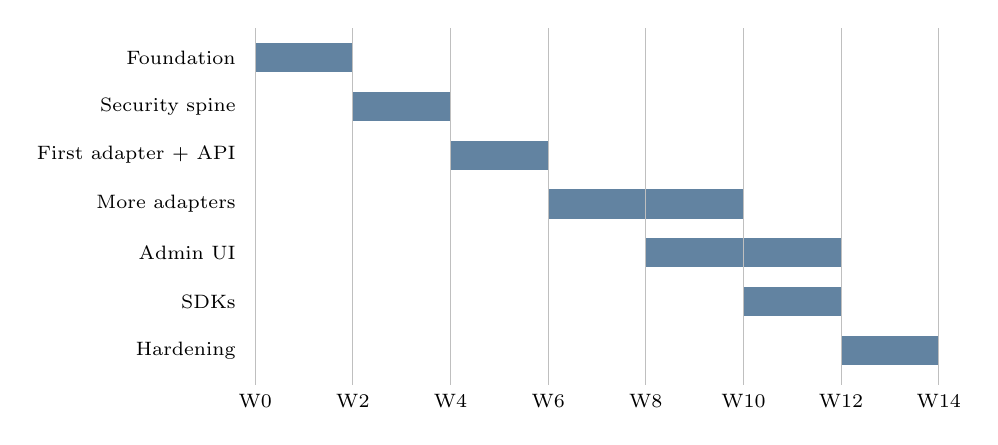
\begin{tikzpicture}[x=0.62cm,y=0.62cm]
  \def\bar#1#2#3#4{\fill[brand!70] (#2,#1) rectangle (#3,#1+0.6); \node[anchor=east,font=\scriptsize] at (-0.2,#1+0.3) {#4};}
  \bar{6}{0}{2}{Foundation}
  \bar{5}{2}{4}{Security spine}
  \bar{4}{4}{6}{First adapter + API}
  \bar{3}{6}{10}{More adapters}
  \bar{2}{8}{12}{Admin UI}
  \bar{1}{10}{12}{SDKs}
  \bar{0}{12}{14}{Hardening}
  \foreach \w in {0,2,...,14}{\draw[black!25] (\w,-0.4) -- (\w,6.9); \node[font=\scriptsize,below] at (\w,-0.4) {W\w};}
\end{tikzpicture}
\caption{MVP plan in weeks.}
\end{figure}

\begin{tabularx}{\linewidth}{@{}>{\raggedright\arraybackslash}p{3.0cm}>{\raggedright\arraybackslash}p{4.8cm}X@{}}
\toprule
\textbf{Phase} & \textbf{Goal} & \textbf{Exit criteria}\\
\midrule
1. Foundation & Repo, core types, adapter protocol, control-plane schema & core builds; migrations apply cleanly\\
2. Security spine & Vault, auth, audit, network guard & Secrets encrypted end to end; SSRF tests pass\\
3. First path & Postgres adapter plus API & Conformance suite green on Postgres\\
4. More adapters & MongoDB, Firestore, MySQL, SQL Server, DynamoDB & Each passes conformance and security suites\\
5. Admin UI & Connect, introspect, edit, permissions & An editor completes a full content edit through the UI only\\
6. SDKs & Generated Dart and Python, hand-tuned TypeScript & Sample apps (Next.js, Flutter, FastAPI) run\\
7. Hardening & Load, security review, docs, cloud identity & Security review and key-rotation drill done\\
\bottomrule
\end{tabularx}\smallskip

\subsection{Hand-written files for the MVP (estimate)}
\begin{tabular}{@{}lr@{\hspace{2.2cm}}lr@{}}
\toprule
\textbf{Area} & \textbf{Files} & \textbf{Area} & \textbf{Files}\\
\midrule
Root config & 12 & api & 25\\
core & 15 & worker & 12\\
protocol + adapter-sdk & 13 & admin & 40\\
6 adapters & 36 & control-plane DB & 10\\
vault & 8 & sdk-ts & 8\\
auth & 10 & Dart SDK & 8\\
audit + network-guard & 11 & Python SDK & 9\\
infra & 15 & adapter templates (Go, Python) & 16\\
tests & 20 & CI + docs & 20\\
\midrule
\multicolumn{3}{@{}l}{\textbf{Total (approximate)}} & \textbf{288}\\
\bottomrule
\end{tabular}

\subsection{Risks}
\begin{tabularx}{\linewidth}{@{}>{\raggedright\arraybackslash}p{5.2cm}X@{}}
\toprule
\textbf{Risk} & \textbf{Mitigation}\\
\midrule
Capability gaps make some databases feel second class & Honest capability flags; clear UI messaging\\
Credential handling mistakes & Security spine before any adapter; key-rotation drill\\
Scope creep across databases & Ship six adapters; add others on demand\\
Driver or ORM version changes (for example Prisma and MongoDB) & No single ORM for all stores; isolate drivers inside adapters\\
Licensing of embedded tools & Prefer MIT/Apache components; legal review before embedding source-available tools\\
\bottomrule
\end{tabularx}\smallskip

%--------------------------------------------------------------------
\appendix
\section{Adapter Protocol (proto)}
\lstinputlisting[language=proto]{../schemas/adapter.proto}

\section{Architecture Decision Records}
\subsection*{ADR 0001: Language choice \hfill\normalfont\small Proposed, 2026-10-08}
\textbf{Decision:} TypeScript for core, adapter-sdk, first-party adapters, api, worker and admin; generated Dart and Python SDKs; adapters in any language through a language-neutral protocol. \textbf{Revisit when} worker CPU or connection counts become the bottleneck, or a customer needs an adapter whose best driver is not on Node.

\subsection*{ADR 0002: Adapters as processes behind a protocol \hfill\normalfont\small Proposed, 2026-10-08}
\textbf{Decision:} define the adapter contract in \code{adapter.proto} and run adapters as separate worker processes, with an in-process fast path for trusted first-party adapters. \textbf{Gains:} any language, per-connection isolation, one conformance kit. \textbf{Costs:} a network hop and more services to operate.

\subsection*{ADR 0003: CMS metadata lives in the control plane \hfill\normalfont\small Proposed, 2026-10-08}
\textbf{Decision:} store all CMS metadata in a separate control-plane Postgres; customer databases hold only customer data; connections are read-only by default. \textbf{Cost:} schema drift must be caught by re-introspection and reconciled with stored metadata.

\end{document}
